% This is ''sig-alternate.tex'' V2.0 May 2012
% This file should be compiled with V2.5 of '\'sig-alternate.cls'' May 2012
%
% This example file demonstrates the use of the \'sig-alternate.cls'
% V2.5 LaTeX2e document class file. It is for those submitting
% articles to ACM Conference Proceedings WHO DO NOT WISH TO
% STRICTLY ADHERE TO THE SIGS (PUBS-BOARD-ENDORSED) STYLE.
% The \'sig-alternate.cls' file will produce a similar-looking,
% albeit, 'tighter' paper resulting in, invariably, fewer pages.

\documentclass{sig-alternate}
\usepackage{paralist}
\usepackage{url}

\begin{document}
%
% --- Author Metadata here ---
\conferenceinfo{WIPSCE}{2015 London, UK}
\CopyrightYear{2015} % Allows default copyright year (20XX) to be over-ridden - IF NEED BE.
%\crdata{0-12345-67-8/90/01}  % Allows default copyright data (0-89791-88-6/97/05) to be over-ridden - IF NEED BE.
% --- End of Author Metadata ---

\title{Technocamps: A Decade of Supporting\\Computer Science Education in Wales}

\numberofauthors{2} 
\author{
% 1st. author
\alignauthor
Tom Crick\\
\affaddr{Department of Computing}\\
\affaddr{Cardiff Metropolitan University, UK}\\
\affaddr{tcrick@cardiffmet.ac.uk}
% 2nd. author
\alignauthor
Faron Moller\\
\affaddr{Department of Computer Science}\\
\affaddr{Swansea University, UK}\\
\affaddr{f.g.Moller@swansea.ac.uk}\\
}

\maketitle

\begin{abstract}
In this paper we will outline the history (and prehistory) of
Technocamps including the changes to computing education in schools
which made Technocamps necessary and timely; explain the evolved
nature of education in the UK focusing on Wales with its specific
challenges and opportunities; and present data both in support of
intervention as well as the positive effect this intervention is
having. The authors both sit on an official Welsh Government Steering
Group (with the first author acting as co-chair) which is to deliver a
report to the Minister in July with recommendations for computer
science curriculum reform; this paper will also present the background
and thinking of this Group.
\end{abstract}

% A category with the (minimum) three required fields
\category{K.3.2}{Computers \& Education}{Computer and Information Science Education}[Computer Science Education]
\category{K.4.1}{Computers And Society}{Public Policy Issues}
\keywords{Computer Science Education; High School; Teachers}


\section*{To Do}

In no particular order...

\begin{itemize}
\item Set UK context over past 3-5 years
\item Link to English and Scottish changes
\item Welsh context
\item Technocamps: the ten year journey from 2003
\item Convergence, the pan-Wales problem
\item Key contributions: aims, targets, impacts, young people, NEETs, coverage
\item Links with CAS Wales
\item Hubs (both TC and CAS)
\item Funding models: ESF, NSA, Nesta, etc
\item {\textbf{Key theme}}: Building capacity, the problems of
  England's NoE model in Wales
\item UK policy: RS report, English curriculum, qualification change,
  UKForCE, etc.
\item Welsh policy: ICT curriculum, ICT review, Estyn reports, ICT
  sector support/economic drivers, curriculum change,
  Donaldson and post-Donaldson
\item THE FUTURE...!
\end{itemize}


\section{Introduction}
Key citations~\cite{crick+sentance:2011,sentance-et-al-wipsce2012,brown-et-al-sigcse2012,brown-et-al-toce2014}.

% taken from TOCE pitch from 2013
In the early 1980s, the BBC Micro was introduced to schools throughout
Britain, and before long they were in 80\% of UK classrooms. By
encouraging young learners to experiment with computers, a generation
of creative (and computational) talent was spawned. Applications in
the UK to study computer science at university hit a peak, and
computer science graduates changed the world as they helped computers
come to dominate every aspect of our lives.

Fast forward 30 years and the situation could not be any more
different. The computer is no longer a novelty. Children now spend
more time at home in front of a computer screen than a TV screen, but
like the TV, their interest is restricted to using the computer, not
in experimenting with it. Computer studies in school (now called
``Information and Communication Technology'' (ICT)) has evolved into IT
studies with an emphasis on digital literacy and office skills --
significantly more mundane than the social networking and gaming for
which the pupils use their home computers. 65\% of IT teachers in the
UK do not have a relevant qualification but have slipped into the role
of IT teacher simply by being digitally literate. Applications to
study computer science at university slumped -- especially amongst
females -- and many of those who start a university computer science
course drop out during the first year as they are unaware of what
computer science is and what studying it entails.

A decade ago, the Department of Computer Science at Swansea University
started looking into ways to address this issue. In 2003 we at Swansea
started Technocamps, a schools outreach programme which brings groups
of school children to the University for day-long workshops based on
selected computational themes to inform them what computing is about,
with follow-up extracurricular clubs (``Technoclubs'') in the
schools. Of course we are not alone in exploring solutions to a
perceived problem in education. In particular, in 2008 the UK-wide
organization Computing At School (CAS) was formed, and its current
membership of over 3000 teachers and computing professionals are
working hard to promote the teaching of computing at school.

Technocamps was very successful as a local initiative, with many
students studying computer science at Swansea claiming to be
influenced by Technocamps activities. In 2010, based on empirical data
regarding its effect on school children's attitudes towards computing
-- as well as their teachers -- Swansea University was awarded £6
million funding by the Welsh Government under the EU's European Social
Fund (ESF) Convergence Programme to run Technocamps as a pan-Wales
project; since then, Technocamps has been operating with regional hubs
at the Universities of Aberystwyth, Bangor, and Glamorgan. Though
focusing on the children, Technocamps also provides "Technoteach"
events aimed at up-skilling IT teachers in Welsh schools. Since 2010,
Technocamps has provided computing-related activities and resources
for thousands of young people across Wales, as well as interacting
with hundreds of teachers at a majority of the nation's schools.

Wales is a devolved nation within the United Kingdom, with its own
elected national government fully responsible for its education
system. The Welsh Government's Minister for Education and Skills has
publicly stated the importance of computer science education and is a
key supporter of Technocamps, understanding the wider educational and
socio-economic impact that his government can make with reform in
Wales. With only 5\% of the population of England but with distinct
socio-cultural challenges, Wales represents an ideal microcosm for
experimenting to effect educational change.

% taken from TOCE paper, can be adapted to Welsh focus
\section{School Systems in the UK}\label{sec:schools}

As reported by Hubweiser et al.~\cite{hubwieser-et-al:2011}, when establishing a
model for viewing school CS education, it is apparent that there is
much diversity between school education systems, and this can create
an obstacle when trying to understand progress made in a different
country. Here we describe the context of school education in the UK.

For historical reasons, the UK does not have a single nationwide
education system.  The UK is primarily composed of four devolved
nations: England (population: 53.0 million), Scotland (5.3 million),
Wales (3.0 million) and Northern Ireland (1.8
million)\footnote{\url{http://www.ons.gov.uk/ons/guide-method/census/2011/index.html}}.
Each nation has its own education system, although they are broadly
similar in England and Wales.

% something brief about Scotland and NI too?
\subsection{England and Wales}
Figure~\ref{fig:key-stages} shows the system of five Key Stages (KS)
used in England and Wales (although KS1 is called Foundation Phase in
Wales) with compulsory schooling until age 16. All subjects are
compulsory until the end of Key Stage 3 (KS3) and then students can
choose approximately ten subjects to study for the next two years,
which each lead to GCSE (General Certificate of Secondary Education)
qualifications. However, while the National Curriculum in England and
Wales are broadly similar, they are distinct and use different
terminology.

\begin{figure}
  \centering
  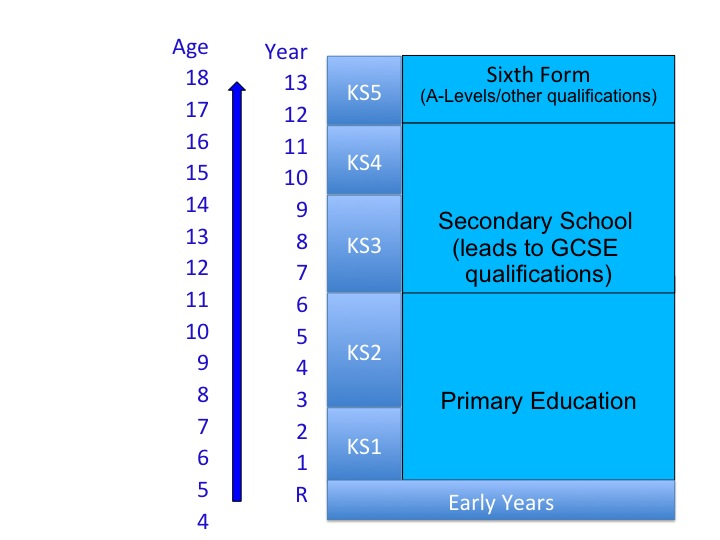
\includegraphics[width=\columnwidth]{images/key-stages.png}
  \caption{Key Stages in the English and Welsh education system}
  \label{fig:key-stages}
\end{figure}

% adjust to be Wales-focused
There is state provision for education in the UK up to the age of 19,
with mostly comprehensive, mixed ability schools across the UK. A few
areas in England have retained a system of selective 11+ schools
called grammar schools, which require students to sit an exam prior to
entry, but these schools are in the minority. As well as state
schools, 10\% of schools in the UK are independent fee-paying
schools. Overall, in England there are approximately 24,000 schools,
including 16,800 primary schools, 3,400 secondary schools and 2,400
independent schools (primary and secondary).  However, the primary and
independent schools tend to be smaller: the state-funded schools had
4.2 million primary pupils and 3.2 million secondary pupils, with 0.6
million pupils in independent schools. The ICT
curriculum in Wales
(2008)\footnote{\url{http://wales.gov.uk/topics/educationandskills/schoolshome/curriculuminwales/arevisedcurriculumforwales/nationalcurriculum/ictnc/?lang=en}},
was perceived to be less prescriptive than the ICT curriculum in
England, but exhibiting many of the same issues. It was recently
reviewed by an independent steering group appointed by the Welsh
Government~\cite{welshictreview:2013}, making clear recommendations for
reforming the ICT curriculum as part of a broader national curriculum
review for September 2014.

\section{Conclusions}
End here...


% bib
\bibliographystyle{abbrv}
\bibliography{wipsce2015}

\end{document}
